\documentclass{standalone}

\usepackage{tikz}
\usepackage{pgfplots}
\pgfplotsset{compat=1.3}
\definecolor{hred}{HTML}{e94b3c}
\definecolor{hblue}{HTML}{6f9fd8}

\begin{document}
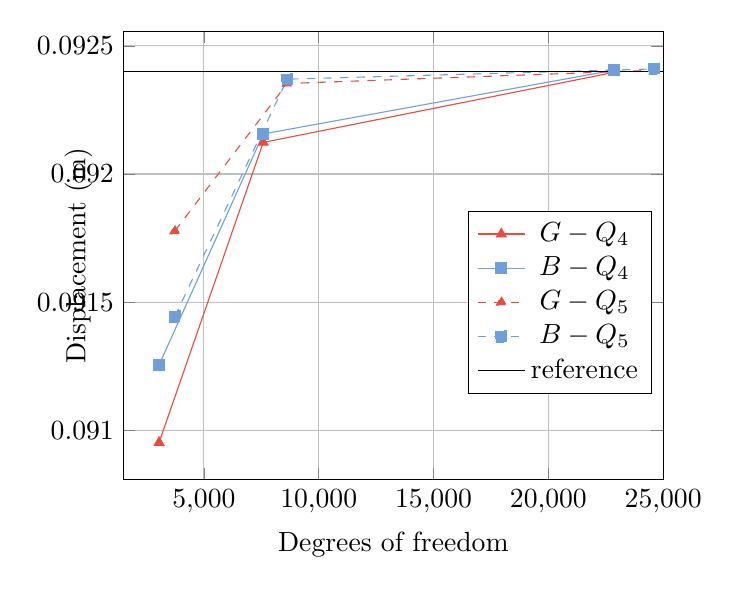
\begin{tikzpicture}
	\begin{axis}[grid=major,xmin=1500,xmax=25000,
			legend style={at={(.98,.6)}},
			transpose legend,
			yticklabel style={scaled ticks=false,
									/pgf/number format/fixed,
									/pgf/number format/precision=5},
			xlabel= Degrees of freedom,
			ylabel=Displacement (m),
			y label style={at={(axis description cs:-0.04,.5)},rotate=0,anchor=south},
		]

		\addplot [mark=triangle*, hred] coordinates {
				(3048,	0.0909526)
				(7584,	0.0921232)
				(22848,	0.0923963)
			};

		\addplot [ mark=square*, hblue] coordinates {
				(3048,	0.0912555)
				(7584,	0.0921563)
				(22848,	0.0924049)
			};

		\addplot [mark=triangle*, hred , dashed] coordinates {
				(3732,	0.0917774)
				(8628,	0.092353)
				(24612,	0.0924045)
			};

		\addplot [mark=square*, hblue, dashed] coordinates {
				(3732,	0.0914439)
				(8628, 	0.0923699)
				(24612,	0.0924099)
			};

		\addplot [black] coordinates {
				(1500,	0.0924)
				(25000,	0.0924)
			};
		\legend{$G-Q_4$\\$B-Q_4$\\$G-Q_5$\\$B-Q_5$\\reference\\}
	\end{axis}
\end{tikzpicture}
\end{document}